\section{Aufgabe 3} \label{ex3}

Konfiguration des IP Cores zur Realisierung der Kommunikation zwischen Prozessor und 
Peripherie als Blockdesign in Vivado 2016.2. Eingebunden in diese wurden zusätzlich die 8Bit-LED-Anzeige und die Push-Buttons. Der Aufbau wurde anschließend in VHDL synthetisiert. 

\begin{minipage}{\textwidth}
    \begin{center}        
        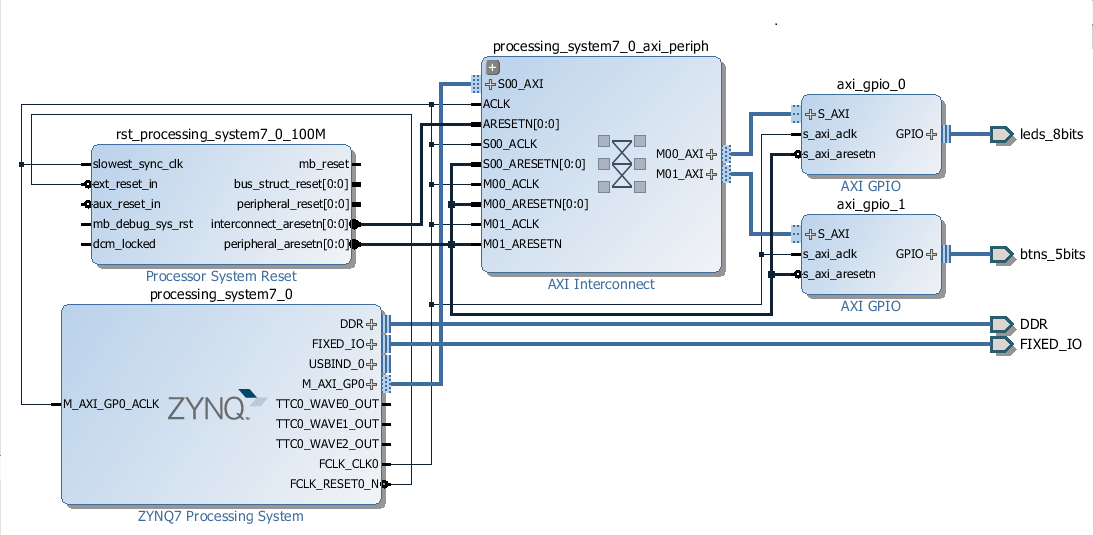
\includegraphics[scale=0.6]{img/a3.png} 
    \end{center}
\end{minipage}
\begin{center}
Vivado: Schemaplan der IP-Cores
\end{center}